\documentclass[10pt,a4paper]{article}
\usepackage[T1]{fontenc}
\usepackage[utf8]{inputenc}
\usepackage{lmodern}
\usepackage[hmargin=16mm,top=15mm,bottom=12mm,headheight=14pt,headsep=4mm,footskip=7mm]{geometry}
\usepackage{microtype,graphicx,booktabs,tabularx,amsmath}
\usepackage[table]{xcolor}
\usepackage{enumitem,caption,fancyhdr,hyperref}
\definecolor{ink}{HTML}{17344A}
\definecolor{accent}{HTML}{087E74}
\definecolor{tablehead}{HTML}{EEF1F3}
\definecolor{tablerule}{HTML}{DDE3E7}
\definecolor{tablefinal}{HTML}{EDF7F4}
\hypersetup{colorlinks=true,urlcolor=accent,linkcolor=ink,pdftitle={Beyond the hourly average},pdfauthor={ApplePi}}
\usepackage{titlesec}
\usepackage{eurosym} 
\usepackage{newunicodechar}
\titleformat{\section}{\large\bfseries\color{ink}}{}{0pt}{}
\titlespacing*{\section}{0pt}{6pt}{3pt}
\setlength{\parindent}{0pt}
\setlength{\parskip}{3.5pt}
\setlist[itemize]{leftmargin=*,topsep=1pt,itemsep=0pt,parsep=0pt}
\captionsetup{font=small,labelfont=bf,skip=5pt}
\pagestyle{fancy}\fancyhf{}
\fancyhead[L]{\small\color{ink}APPLEPI\quad /\quad AET NEURAL WAVE 2026}
\fancyhead[R]{\small Project report}
\fancyfoot[R]{\small\thepage\ /\ 3}
\renewcommand{\headrulewidth}{0.3pt}
\begin{document}
{\LARGE\bfseries\color{ink} Beyond the hourly average}\par
{\large Quarter-hour price reconstruction for AET}
\vspace{0pt}

\section{The challenge}
Our assigned AET challenge was to reconstruct \textbf{96 quarter-hour electricity prices from 24 supplied hourly prices}, for each of four market zones. The four reconstructed prices within every hour must average back to the supplied hourly price, within a tolerance of \textbf{0.0001 \euro{}/MWh}.

An hourly average hides movements between its four quarters. This matters because electricity is not necessarily delivered evenly throughout the hour, so a more detailed price curve could support more accurate valuation. Our task was to recover as much of that missing shape as possible using the official price data, while keeping the hourly reference unchanged.

\section{Approach}
For hour $h$ and quarter $q$, our prediction is a smooth baseline plus 80\% of a learned correction:
{\setlength{\abovedisplayskip}{1pt}\setlength{\belowdisplayskip}{0pt}\[
\hat p_{h,q} = \underbrace{b_{h,q}}_{\text{PCHIP baseline}} + \, 0.8\,\underbrace{\big(c^{\mathrm{slope}}_{h}\,s_q + c^{\mathrm{curv}}_{h}\,k_q + c^{\mathrm{zig}}_{h}\,z_q\big)}_{\text{LightGBM correction}}.
\]}

Repeating the hourly price four times is the simplest option; smooth interpolation is a better starting point but misses sharper movements within hours. We therefore combined PCHIP (Piecewise Cubic Hermite Interpolating Polynomial) interpolation on the cumulative hourly curve with three LightGBM models. PCHIP provides a shape-preserving baseline that respects hourly averages. LightGBM uses boosted decision trees to learn the remaining corrections from price and calendar features. This gives us a compact model whose output can be explained through three components:
\begin{itemize}
\item \textbf{Slope:} whether prices rise or fall within the hour.
\item \textbf{Curvature:} whether the middle quarters sit above or below the outer quarters.
\item \textbf{Zigzag:} alternating movements between quarters.
\end{itemize}
The shapes $s$, $k$, $z$ add up to zero within each hour, so the corrections change its shape, not its average.

The models use the supplied hourly curves, differences between zones, calendar information and earlier price patterns. They never receive the actual quarter-hour prices of the day being reconstructed. We train each LightGBM model to minimise absolute error on its basis coefficient. We select between candidate configurations using the official mean absolute error on reconstructed quarter-hour prices. Applying 80\% of the learned correction worked better during development than applying it in full, so we kept that setting.

Finally, three fixed rules (no fitted parameters) adjust each hour without changing its average:
\begin{itemize}
\item \textbf{Zone coupling:} zones with almost the same hourly price (within 0.1~\euro{}/MWh) usually move together, so they share one shape: the average of their predicted shapes.
\item \textbf{Partial tie:} zones within 5~\euro{}/MWh behave similarly but less reliably, so each moves 40\% towards the group's shape.
\item \textbf{Sign rule:} quarters rarely change sign within an hour. In a positive hour no quarter may fall below $-0.01$~\euro{}/MWh, in a negative hour none may exceed 0; the remaining quarters shift to keep the average.
\end{itemize}
Together, the rules reduced development MAE by 1.5\% (all eight folds improved). A final adjustment removes floating-point drift, and automated checks confirm the tolerance.

Our official-data EDA highlighted the importance of slope and motivated a stronger linear-ramp benchmark. Evening ramp hours remained difficult, so we also investigated whether additional shape features could help.

\section{Challenges and solutions}
\textbf{Working with incomplete information.} Several quarter-hour profiles can have the same hourly average. We could learn recurring patterns, but we could not expect to recover every movement exactly. This helped us understand the limits of the task.

\looseness=-1 \textbf{Keeping the comparison fair.} We used chronological validation and historical inputs matched by calendar date. This prevents missing dates from shifting the history and keeps the target day's quarter-hour observations out of the model inputs.

\looseness=-1 \textbf{Exploring different model families.} We tested Ridge and CatBoost, as well as temporal CNN, dilated TCN, LSTM and Transformer models. For the baseline-plus-correction approach, we compared LightGBM with CatBoost, Ridge, Random Forest and Extra Trees. We also explored different interpolation methods, correction weights and separate models for each zone.

\looseness=-1 \textbf{Deciding when to stop adding complexity.} Local-geometry features slightly worsened development MAE from \textbf{3.9479 to 3.9497 \euro{}/MWh}, so we retained the existing features. We also explored temporal and Bayesian graph models, error-correction models and ensembles. In a separate \textbf{June--August window}, a 25\% compact-graph / 75\% reference-model blend reduced MAE from \textbf{4.2246 to 4.2058 \euro{}/MWh} (0.4\%). We kept LightGBM, as this small gain did not justify the added complexity.

\newpage
\section{Results}
We evaluated the model using mean absolute error (MAE), the average distance between reconstructed and observed prices. Each evaluation day and zone has equal weight; lower values are better.

For development, we used eight chronological January--August folds, training on earlier dates and scoring days 19 through month-end. We then assessed a model trained through 31 August on 19--30 September. September results are also available for the graph experiments, and we scored September again before switching to the final rules, so we report this as a historical assessment rather than an untouched final test.

\textbf{Overall reconstruction accuracy}
\begin{center}
\setlength{\tabcolsep}{10pt}
\renewcommand{\arraystretch}{1.35}
\arrayrulecolor{tablerule}
\begin{tabularx}{\linewidth}{*{3}{>{\raggedright\arraybackslash}X}}
\rowcolor{tablehead}
\textbf{Method} & \textbf{Development MAE} & \textbf{September MAE}\\\hline
Flat hourly prices & 8.13 & 10.90\\\hline
PCHIP & 5.62 & 6.93\\\hline
Full correction (scale 1.0) & 3.98 & 5.43\\\hline
Scaled correction, no rules & 3.95 & 5.04\\\hline
\rowcolor{tablefinal}
\textbf{Final model} & \textbf{3.89} & \textbf{5.00}\\\hline
\end{tabularx}
\captionof{table}{Average price error in \euro{}/MWh{}, from the project results summary. Development covers January--August folds. September scores, including PCHIP, use the same 19--30 September window. The full correction and the version without rules are comparisons, not the submitted model.}
\end{center}

\vspace{4pt}
\textbf{By zone (September assessment)}
\begin{center}
\setlength{\tabcolsep}{10pt}
\renewcommand{\arraystretch}{1.3}
\arrayrulecolor{tablerule}
\begin{tabularx}{\linewidth}{*{4}{>{\raggedright\arraybackslash}X}}
\rowcolor{tablehead}
\textbf{Zone} & \textbf{Model MAE} & \textbf{Flat MAE} & \textbf{Error reduction}\\\hline
ZONE\_0 & 3.83 & 10.78 & \textcolor{accent}{64.5\%}\\\hline
ZONE\_1 & 6.12 & 13.30 & \textcolor{accent}{54.0\%}\\\hline
ZONE\_2 & 5.49 & 9.72 & \textcolor{accent}{43.5\%}\\\hline
ZONE\_3 & 4.57 & 9.79 & \textcolor{accent}{53.3\%}\\\hline
\end{tabularx}
\captionof{table}{September average price error by zone, comparing the final model with repeating the hourly price.}
\end{center}

The final model reduces average price error by \textbf{52.2\% on development dates} and \textbf{54.1\% on the September assessment}, compared with flat prices. Improvements appear in all four zones, although their size varies. Compared with the version without rules, the September gain is smaller (0.8\%), and ZONE\_3 is slightly worse (4.57 instead of 4.55).

\begin{center}
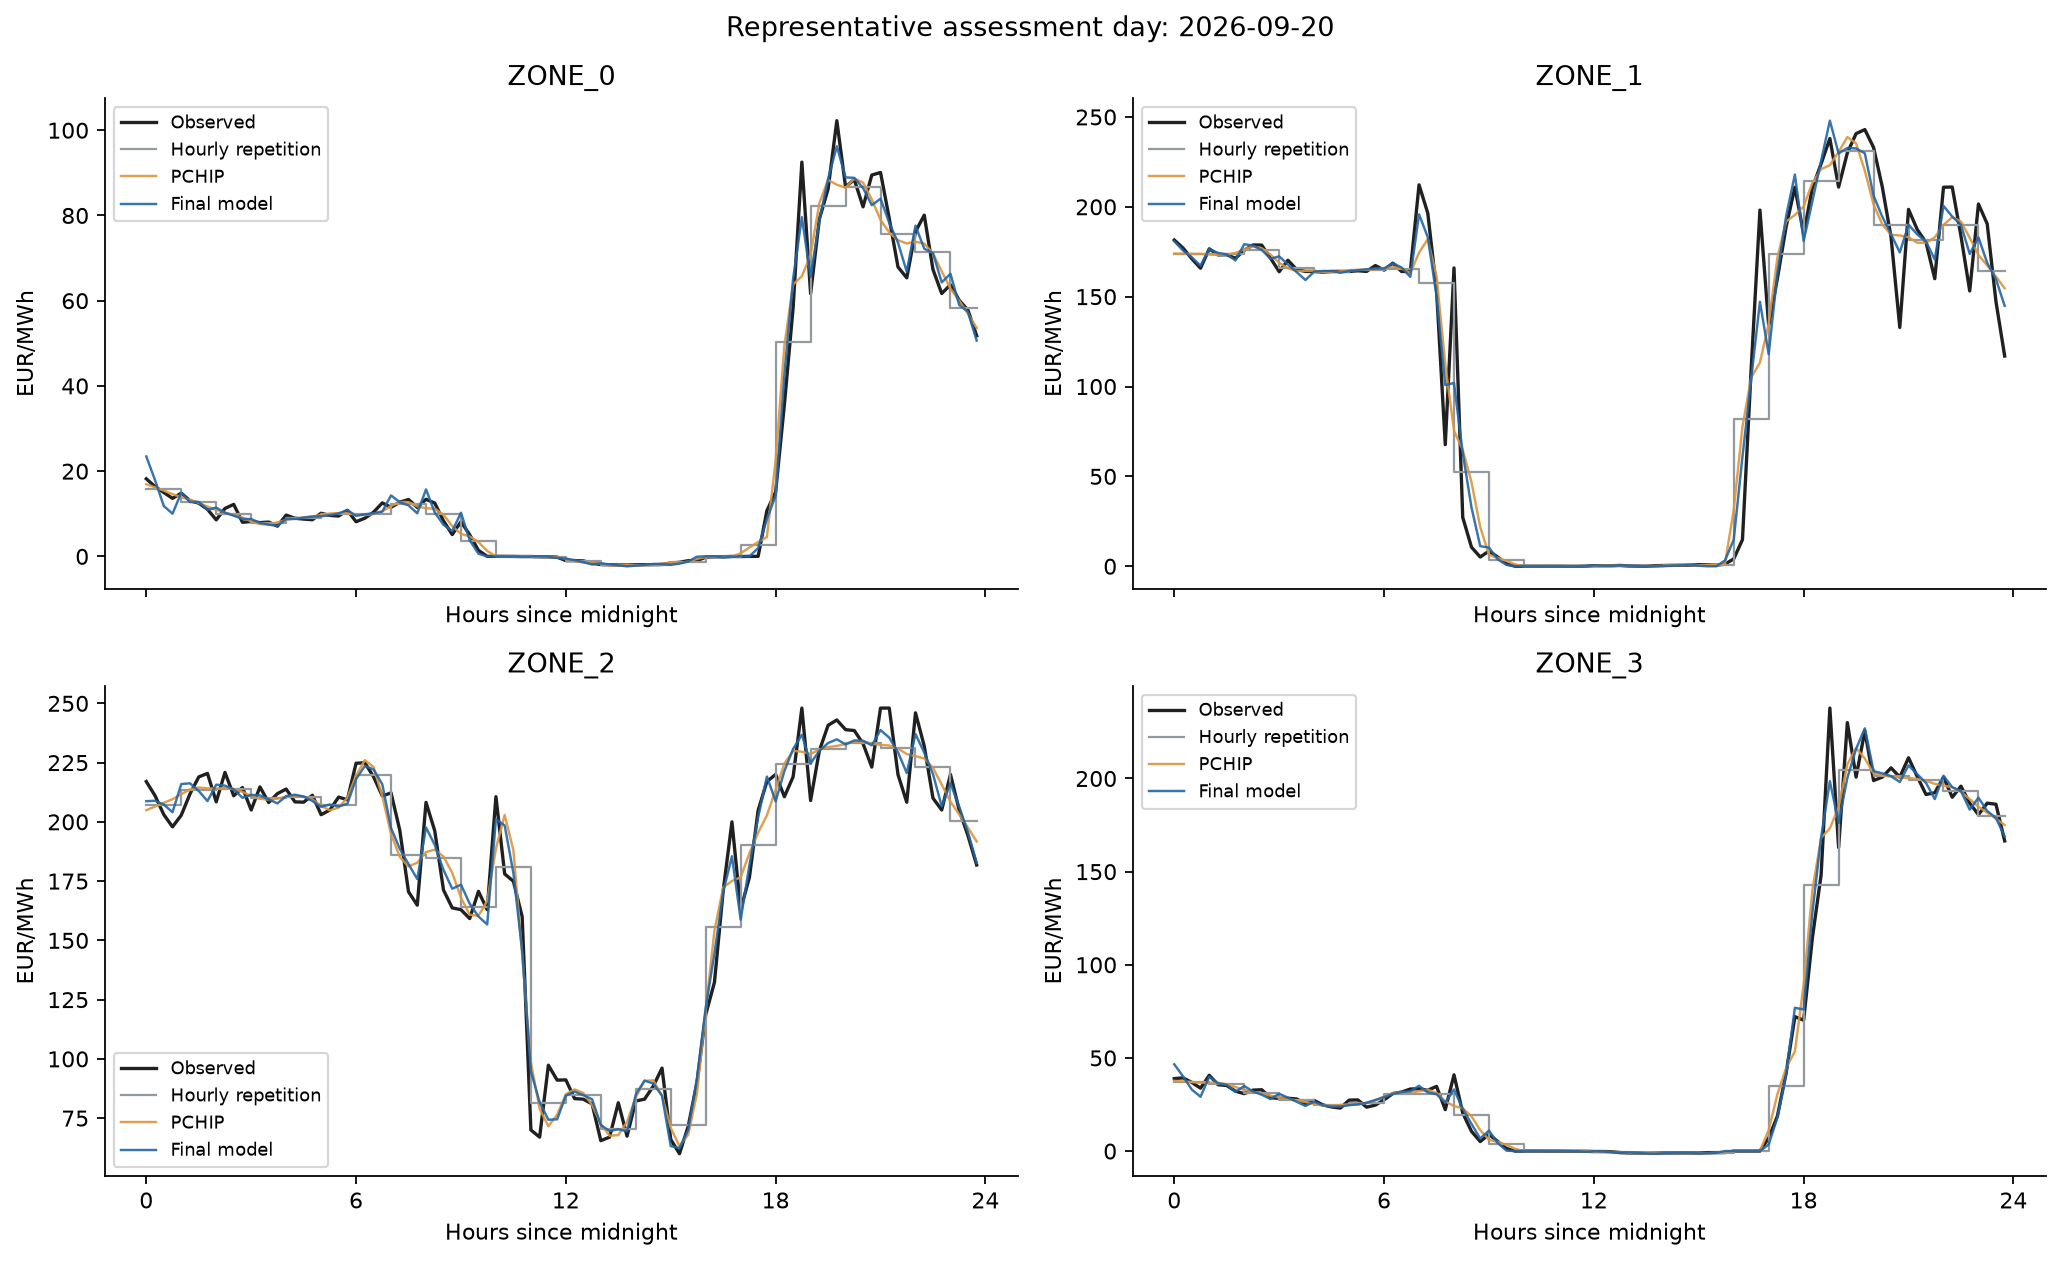
\includegraphics[width=0.67\linewidth]{images/representative_reconstruction.png}
\captionof{figure}{Reconstruction on 20 September 2026 across the four zones. Observed quarter-hour prices are compared with hourly repetition, PCHIP and the final model.}
\end{center}

For us, these results suggest that there is useful structure to recover beyond the hourly average. However, we evaluated price accuracy; we have not measured the effect on actual trading results or portfolio valuations.

\newpage
\section{Dashboard: understanding the predictions}
We also wanted to make the model more approachable for someone who does not work with machine learning. We built an interactive dashboard where users can select a zone and date range and compare reconstructed and observed prices. They can inspect how slope, curvature, zigzag and the final rules contribute to each quarter-hour prediction, and see which signal drove the risk flag for that hour.

\begin{center}
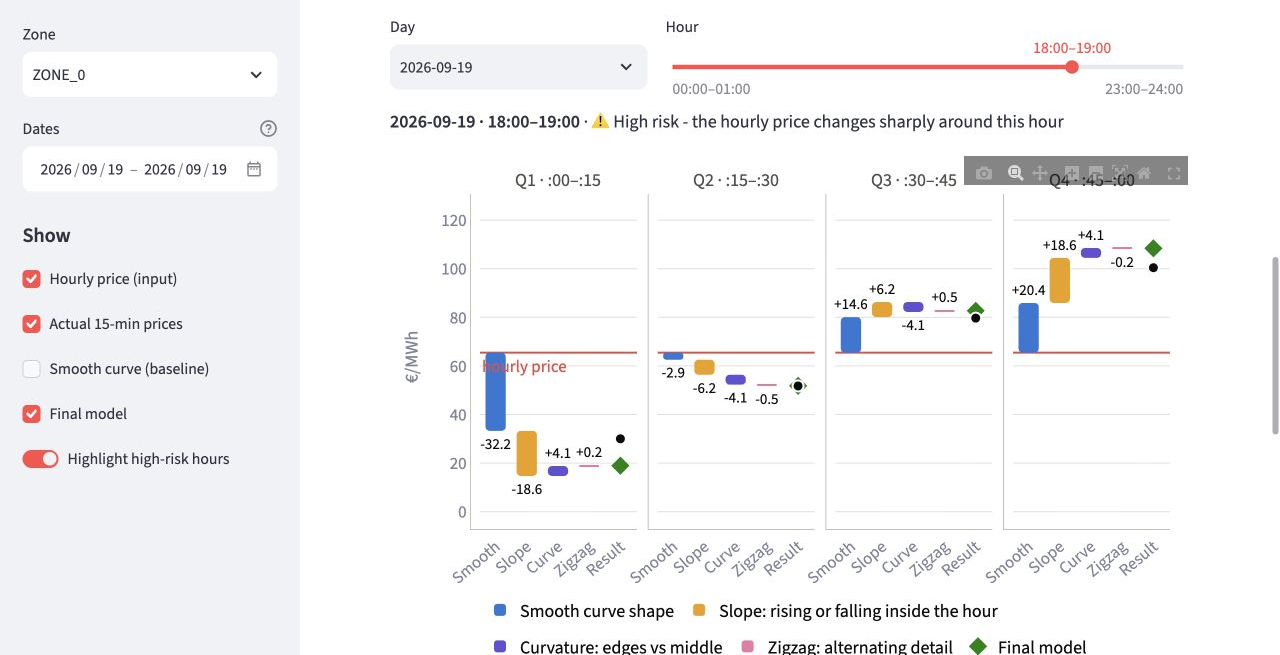
\includegraphics[width=0.82\linewidth]{images/dashboard_detail.png}
\captionof{figure}{Actual dashboard view for ZONE\_0 on 19 September 2026, 18:00--19:00.}
\end{center}

What we find useful about this view is that it shows what happens behind the final curve. Users can see how the baseline, slope, curvature, zigzag and rules contribute to each prediction, including where the model still makes mistakes.

Furthermore, the dashboard highlights potentially difficult hours using hourly ramps, daily price variability and recent historical reconstruction difficulty. These flags explain the main signal behind the label. They are \textbf{heuristics, not calibrated confidence probabilities}, and the dashboard shows a historical assessment replay.

\subsection*{Does the indicator identify harder hours?}
On the January--August development folds, hours flagged as high-risk had \textbf{2.8--3.9 times the reconstruction error} of low-risk hours across the four zones. This suggests that the indicator helps distinguish harder hours, although it does not guarantee an individual prediction's accuracy.

\begin{center}
\setlength{\tabcolsep}{8pt}
\renewcommand{\arraystretch}{1.2}
\arrayrulecolor{tablerule}
\begin{tabularx}{\linewidth}{*{4}{>{\raggedright\arraybackslash}X}}
\rowcolor{tablehead}
\textbf{Zone} & \textbf{Low-risk MAE} & \textbf{High-risk MAE} & \textbf{High / low}\\\hline
ZONE\_0 & 1.51 & 5.89 & 3.9$\times$\\\hline
ZONE\_1 & 2.80 & 8.32 & 3.0$\times$\\\hline
ZONE\_2 & 2.03 & 5.68 & 2.8$\times$\\\hline
ZONE\_3 & 2.22 & 7.20 & 3.2$\times$\\\hline
\end{tabularx}
\captionof{table}{Observed reconstruction MAE in \euro{}/MWh{} by risk group on the development folds.}
\end{center}

\section{AI agents and LLM usage}
We worked with LLM-based coding assistants throughout the project, especially when coding. It was an iterative process: we tried an approach, looked at the results, and used the assistants to help identify errors and work through possible solutions. We also discussed our EDA findings with them to explore which features or model changes might be worth testing. We then checked those suggestions through tests and backtesting, keeping the changes that improved the results. Finally, we used them to help organise and revise the repository, report and presentation, refining the explanations through several rounds of feedback.

\section{More Information}
The papers, libraries and challenge materials we consulted are listed in \texttt{docs/REFERENCES.md} in the repository, including references related to the approaches we tested but did not retain.
\end{document}
